\documentclass{article}
\usepackage[top=2.54cm, bottom=2.54cm, left=2.54cm, right=2.54cm]{geometry}
\usepackage{graphicx,color,url,amsmath}
\usepackage{enumerate}
\setlength{\parskip}{12pt}
\setlength{\parindent}{0pt}
\begin{document}

\begin{center} Huilin Tong\\
ID:1261574
\end{center}

{\bf Discussion}\\
\begin{enumerate}
\item Ratio is large when the reaction-rate combinations that worked well.

It match the discussion in class for about $10000$ times larger for the correct combination.

$dF$, $dR$, $bR$ these three reaction rates were always bigger than others.

When $eR=dF=0$, tends to irreversible reaction.

\item The entire program runs in $15$s roughly. There is $625$ different combinations, so each combination roughly take $0.024$s.

If 5 values of 10 reaction rates, then have $5^{10}=9,765,625$ combinations. Each combination cost $0.024$s. Total time is $9,765,625 \cdot 0.024 = 234,375$s, $61$ hours.

Not feasible for such situation since it will take too much time to compute the best combination.

\item Decay is that $mRNA\cdot tRNA*$ converts to $mRNA+tRNA$ and back to $mRNA\cdot tRNA*$. $dF*mRNA*tRNA - dR*EB$ is the derivative of decay over time.
\end{enumerate}

{\bf Extra credit}\\


\begin{center}
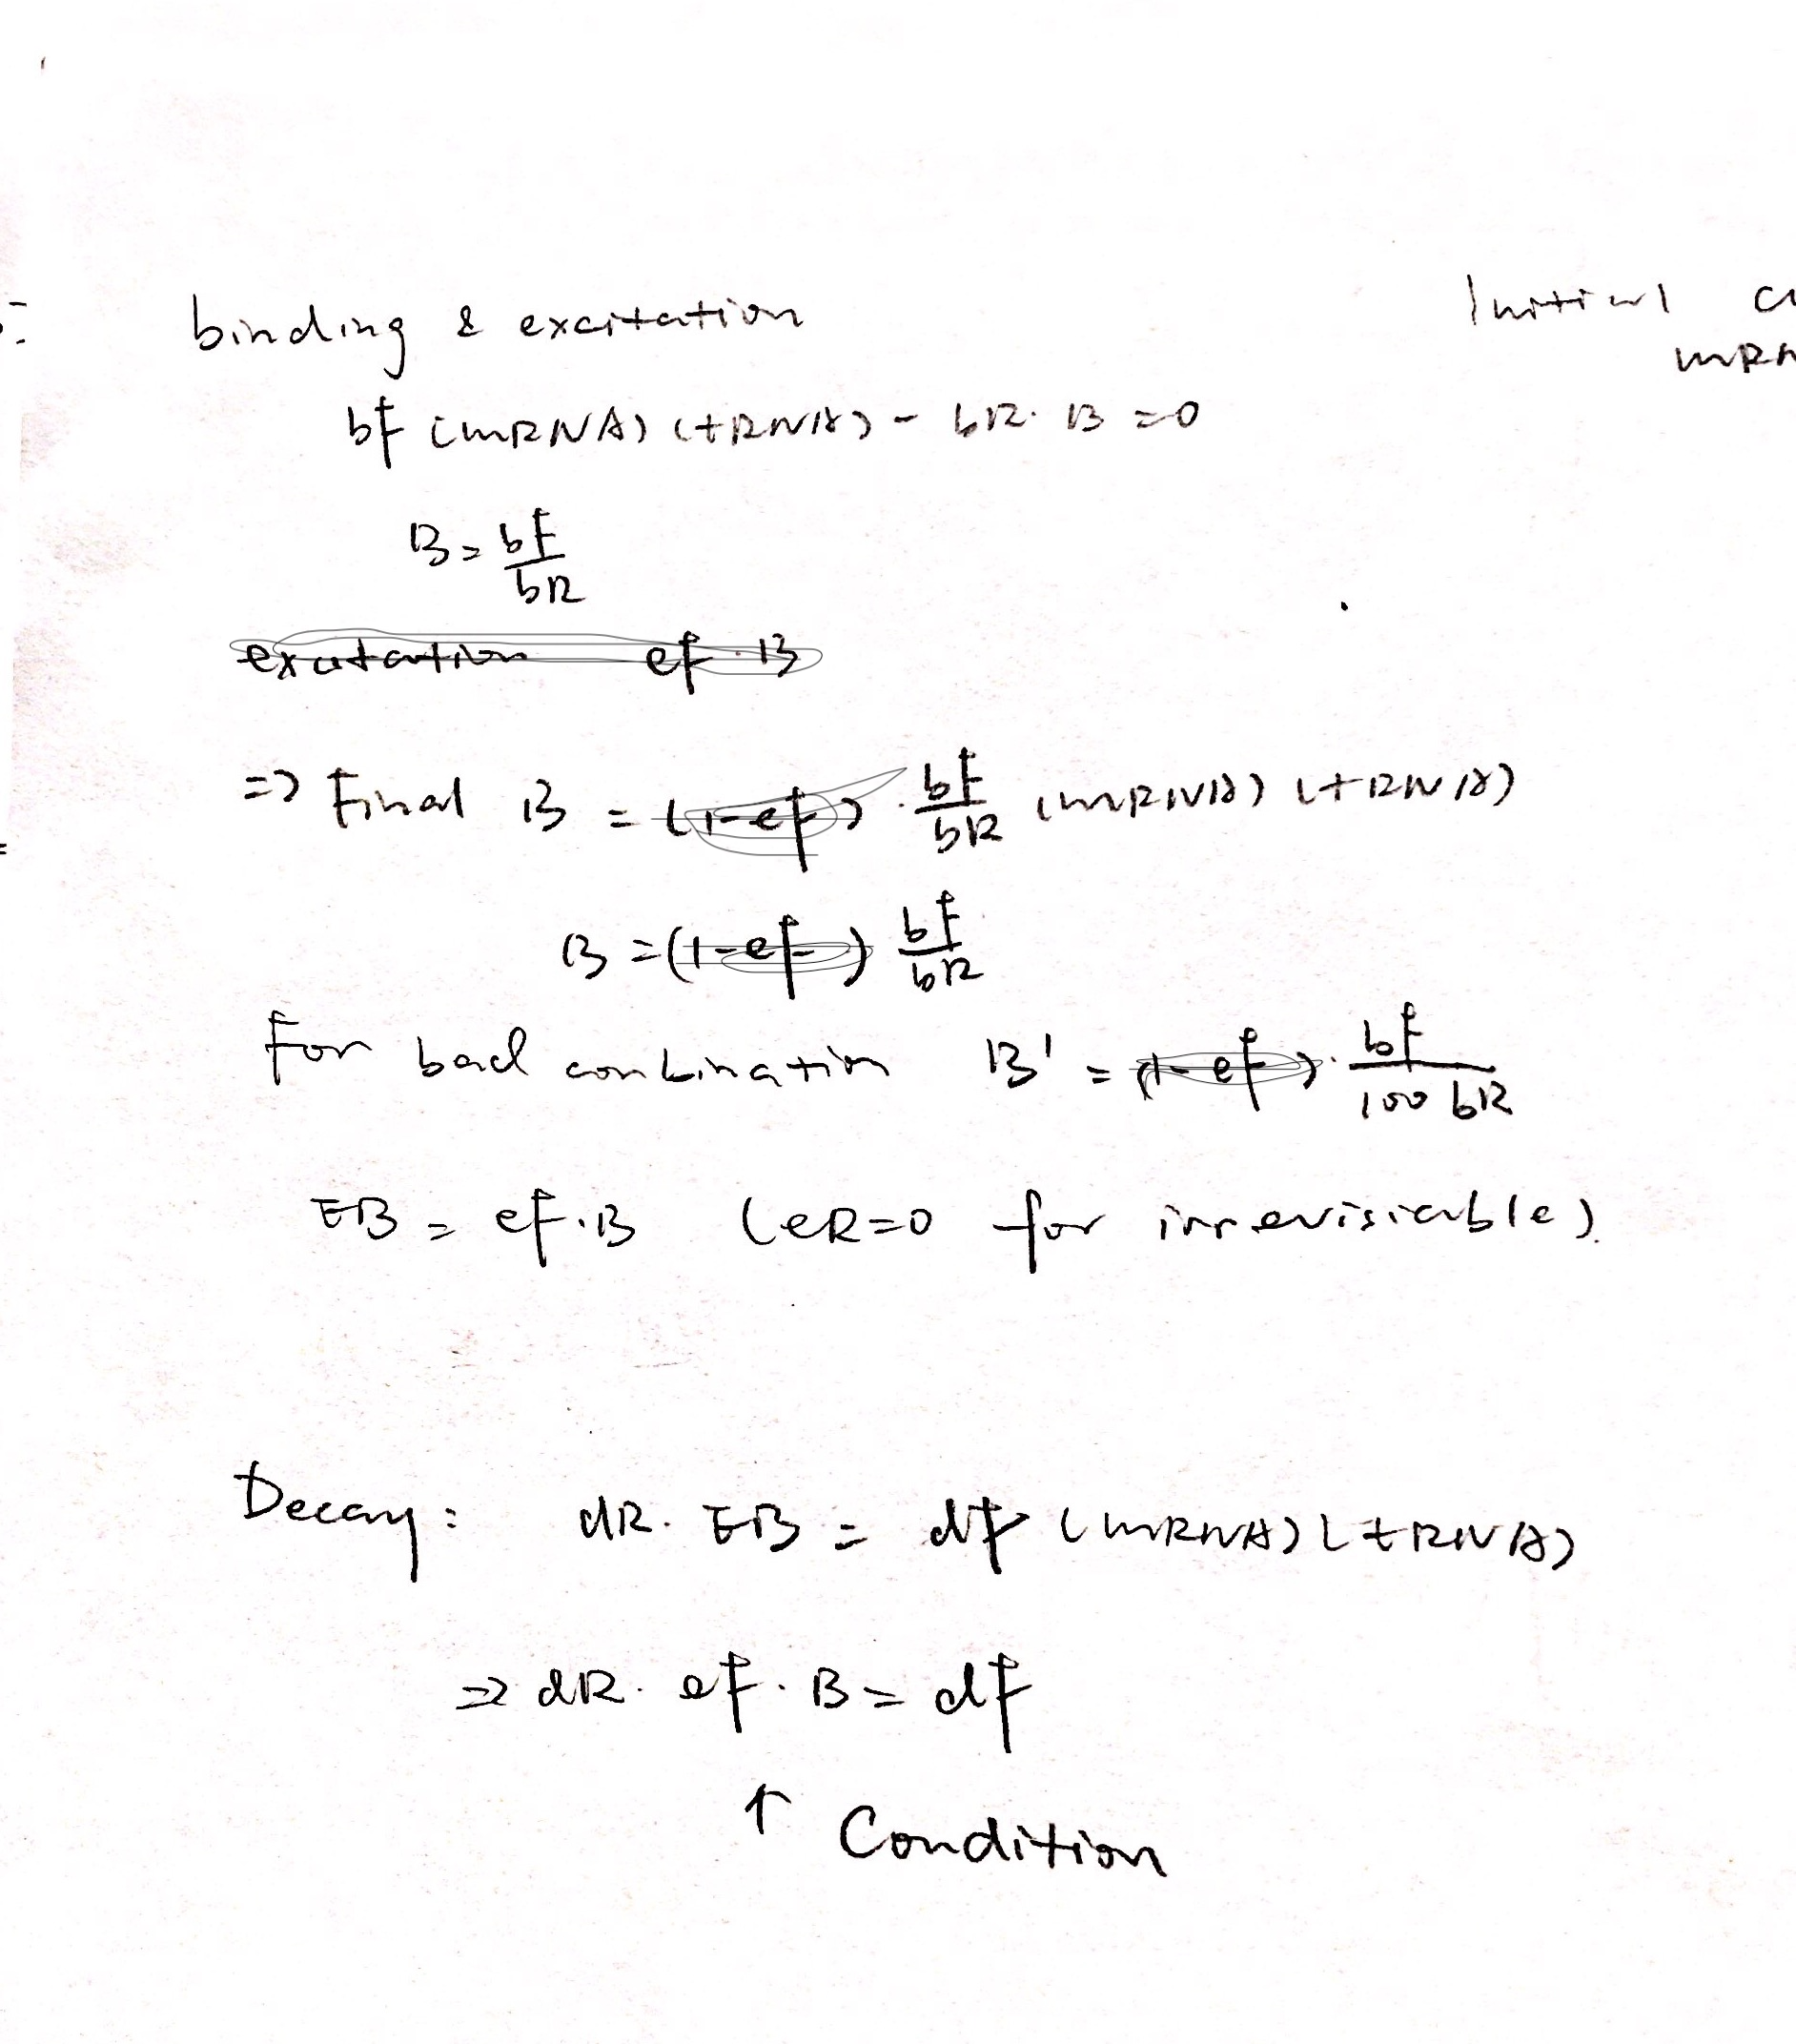
\includegraphics[scale=0.15]{extra.png}	
\end{center}

\end{document}